\chapter{Evaluation \todomatthew{unfinished}}\label{chap:evaluation}

The goal of (dynamic) texture synthesis is to generate 
samples that are indistinguishable from the real input target
texture by a human observer.
In this chapter, a variety of synthesis results are presented,
including qualitative comparisons with competing methods and a user study to quantitatively evaluate the realism
of the results.
Given their temporal nature, the results are best viewed as 
videos.
The two-stream architecture was implemented using TensorFlow
\cite{tabadi2015tensorflowlong}, an open source machine learning framework.
Results were generated using an NVIDIA Titan X (Pascal) GPU
and synthesis times ranged between one to three hours 
to generate $12$ frames with an image resolution of 
$256 \times 256$.
For the full synthesis results and source code, please refer to the
supplemental material. \todomatthew{link website?}

\section{Qualitative results}\label{sec:qualitative_results}

In this section, a qualitative analysis is performed on the tasks of dynamic texture synthesis, incremental texture synthesis,
temporally-endless texture synthesis, and dynamics style transfer.

\subsection{Dynamic texture synthesis}

The dynamic texture synthesis process was applied 
to a wide range of textures which were selected from the 
DynTex \cite{peteri2010} database and others that were collected in
the wild.
Included in the supplemental material are synthesized results
of nearly 60 different textures that encapsulate a range of
phenomena, such as flowing water, waves, clouds, fire, rippling
flags, waving plants, and schools of fish.
Some sample frames are shown in Fig.\ \ref{fig:successes}
but readers are encouraged to view the videos to fully appreciate
the results.

Fig.\ \ref{fig:successes} shows some example success cases with the
two-stream method where appearance and dynamics characteristics from the
target are reliably preserved in the synthesized result. The
upward motion and flickering appearance of \path{fireplace_1}, the outward
motion of the explosive splash of \path{lava},
the wispy fluid dynamics of \path{smoke_1}, the translating god rays and
flowing vegetation of \path{underwater_vegetation_1}, and the downward 
rippling flow of \path{water_3}.

\begin{figure*}[t]
\begin{center}
\begin{tabular}{ >{\centering\arraybackslash} m{0.74in} || >{\centering\arraybackslash} m{5.2in} }

{\footnotesize \texttt{fireplace\_1}\break(original)} &
\showtexture{fireplace_1/frame_} \\
\hline
{\footnotesize \texttt{fireplace\_1}\break(synthesized)} &
\showtexture{fireplace_1_output/frame_} \\

\hline \hline
{\footnotesize \texttt{lava}\break(original)} &
\showtexture{lava/frame_} \\
\hline
{\footnotesize \texttt{lava}\break(synthesized)} &
\showtexture{lava_output/frame_} \\

\hline \hline
{\footnotesize \texttt{smoke\_1}\break(original)} &
\showtexture{smoke_1/frame_} \\
\hline
{\footnotesize \texttt{smoke\_1}\break(synthesized)} &
\showtexture{smoke_1_output/frame_} \\

\hline \hline
{\footnotesize \texttt{underwater}\break\texttt{vegetation\_1}\break(original)} &
\showtexture{underwater_vegetation/frame_} \\
\hline
{\footnotesize \texttt{underwater}\break\texttt{vegetation\_1}\break (synthesized)} &
\showtexture{underwater_vegetation_output/frame_} \\

\hline \hline
{\footnotesize \texttt{water\_3}\break(original)} & 
\showtexture{water_3/frame_} \\
\hline
{\footnotesize \texttt{water\_3}\break(synthesized)} & 
\showtexture{water_3_output/frame_} \\
\end{tabular}
\end{center}
\vspace{-0.45cm}
\caption[Dynamic texture synthesis success examples.]{Dynamic texture synthesis success examples. Names correspond
to files in the supplemental material.}
 \label{fig:successes}
\end{figure*}


\subsubsection{Failure modes}

Example failure modes of the two-stream method are presented in Fig.\ 
\ref{fig:failures}.
In general, most failures result from inputs that
violate the underlying assumption of a dynamic texture, \ie, 
the appearance and/or dynamics are not spatiotemporally homogeneous.
In the case of the \path{escalator} example, the long edge 
structures in the appearance are not spatially homogeneous, 
and the dynamics vary due to perspective effects that
change the motion from purely downward to downward and outward.
The resulting synthesized texture captures an overall downward 
motion but lacks the perspective effects and is unable to 
consistently reproduce the long edge structures.
This is consistent with previous observations
on static texture synthesis \cite{gatys2015} and suggests it is a 
limitation of the local nature of the Gram matrix representation used
in the appearance stream.

Another example is the \path{flag} sequence where the rippling 
dynamics are relatively homogeneous across the pattern but the 
appearance varies spatially.
As expected, the generated texture does not faithfully
reproduce the appearance; however, it does exhibit plausible 
rippling dynamics.

Also shown in Fig.\ \ref{fig:failures} is the \path{cranberries} sequence, which consists of a combination of swirling and wave dynamics.
The model faithfully reproduces the appearance
but is unable to capture the spatially varying dynamics.
Interestingly, it still produces a result
which is statistically indistinguishable from real in the user 
study discussed in Sec.\ \ref{sec:user_study}.

\begin{figure}[t]
\begin{center}
\begin{tabular}{ >{\centering\arraybackslash} m{0.16\textwidth} || >{\centering\arraybackslash} m{0.80\textwidth} }
{\footnotesize \path{escalator}\break(original)} & 
\showtexture{escalator/frame_} \\
\hline
{\footnotesize \path{escalator}\break(synthesized)} & 
\showtexture{escalator_output/frame_} \\
\hline \hline
{\footnotesize \path{flag}\break(original)} &
\showtexture{flag/frame_} \\
\hline
{\footnotesize \path{flag}\break(synthesized)} &
\showtexture{flag_output/frame_} \\
\hline \hline
{\footnotesize \path{cranberries}\break(original)} &
\showtexture{cranberries/frame_} \\
\hline
{\footnotesize \path{cranberries}\break(synthesized)} &
\showtexture{cranberries_output/frame_} \\
\end{tabular}
\end{center}
\vspace{-0.45cm}
\caption[Dynamic texture synthesis failure examples.]{Dynamic texture synthesis failure examples. In
these cases, the failures are attributed to either the
appearance or the dynamics not being homogeneous.}
\label{fig:failures}
\end{figure}

\subsubsection{Appearance vs.\ dynamics streams}

Two experiments were held to verify that the appearance and dynamics
streams were capturing complementary information.
To validate that the texture generation of multiple frames
would not induce dynamics consistent with the input, frames were generated
starting from randomly generated noise but only using the
appearance statistics and corresponding loss, \ie,
Eq.\ \ref{eq:apploss}.
As expected, this produced frames that were valid textures but
with no coherent dynamics present.
Results for a sequence containing a school of fish are shown in
Fig.\ \ref{fig:appearance_only}; to examine the dynamics, see 
\path{fish} in the supplemental material.

Similarly, to validate that the dynamics stream did not 
inadvertently include appearance information, dynamic textures were synthesized
using the dynamics loss only, \ie, Eq.\ \ref{eq:dynloss}.
The resulting frames had no visible appearance and had
an extremely low dynamic range, \ie, the standard
deviation of pixel intensities was 10 for values in $[0,255]$. \todomatthew{maybe include?}
This indicates a general invariance to appearance and 
suggests that the two-stream dynamic texture representation
has factored appearance and dynamics, as desired.

\begin{figure}[t]
\begin{center}
\begin{tabular}{ >{\centering\arraybackslash} m{0.16\textwidth} || >{\centering\arraybackslash} m{0.80\textwidth} }
{\footnotesize target (\path{fish})} & 
\showtexture{fish/frame_} \\
\hline \hline
{\footnotesize appearance only} &
\showtexture{fish_spatialonly/frame_} \\
\hline
{\footnotesize both streams} & 
\showtexture{fish_output/frame_} \\
\end{tabular}
\end{center}
\vspace{-0.45cm}
\caption[Dynamic texture synthesis versus texture synthesis]{Dynamic texture synthesis versus texture synthesis.
(top row) Target texture.
(middle)
Texture synthesis without dynamics constraints shows
consistent per-frame appearance but no temporal coherence.
(bottom)
Including both streams induces consistent appearance and dynamics.
}
\label{fig:appearance_only}
\end{figure}



\subsection{Incremental texture synthesis}

Some example dynamic textures synthesized incrementally, as described in Sec.\ \ref{sec:incremental_synthesis}, are shown in Fig.\ \ref{fig:incremental_synthesis}. \todomatthew{include figure of results}
The resulting textures are perceptually indistinguishable from those
synthesized with the batch process. Included in the supplemental material are synthesized sequences as long as 122 frames (using 11 frame subsequences) with no observed divergence or degradation.

\subsection{Temporally-endless texture synthesis}

An example of a synthesized temporally-endless dynamic texture is shown in
Fig.\ \ref{fig:temporally_endless_synthesis}. As described in Sec.\ 
\ref{sec:temporally_endless_synthesis}, the dynamic texture appears
temporally endless, \ie, there is no explicit beginning or end.
\todomatthew{provide figure showing how it works}

\subsection{Dynamics style transfer}

A dynamics style transfer result is shown in Fig.\ 
\ref{fig:motiontransfer} (top), using two real videos as the appearance and dynamics target, respectively.
Additional examples are available in the supplemental material. \todomatthew{maybe show all examples in thesis?}
When performing dynamics style transfer it is important
that the appearance structure of both targets to be similar in scale and semantics,
otherwise, the generated dynamic textures will look unnatural.
For instance, transferring the dynamics of a flame onto a water 
scene will generally produce implausible results. \todomatthew{show example of this failure case?}

The dynamics of a texture can also be applied to a static input image,
as the target Gram matrices for the appearance loss can be computed
on just a single frame.
This allows us to effectively animate regions of a static image.
The result of this process can be striking and is visualized in
Fig.\ \ref{fig:motiontransfer} (bottom), where the appearance is 
taken from a painting and the dynamics from a real world video.

\begin{figure}[t]
\begin{center}
\begin{tabular}{ >{\centering\arraybackslash} m{0.16\textwidth} || >{\centering\arraybackslash} m{0.80\textwidth} }
appearance target &
synthesized output \\
\hline \hline
\vspace{0.1cm}\showtexframe{water_img.jpeg} &
\showtexture{water_4_to_water_img_output/frame_} \\
\hline
\vspace{0.1cm}\showtexframe{fire_paint.jpeg} &
\showtexture{fireplace_1_to_fire_paint_output/frame_} \\
\end{tabular}
\end{center}
\vspace{-0.45cm}
\caption[Dynamics style transfer.]{Dynamics style transfer.
(top row) 
Appearance of still water was
used with the dynamics of a different water dynamic texture
(\path{water_4}).
(bottom row) 
The appearance of a painting of fire was used
with the dynamics of a real fire (\path{fireplace_1}).
Animated results and additional examples are available in
the supplemental material.} 
\label{fig:motiontransfer}
\end{figure}

\section{User study}\label{sec:user_study}

Quantitative evaluation for (dynamic) texture synthesis is a particularly
challenging task as there is no single correct output when 
synthesizing new samples of a texture.
Like in other image generation tasks (\eg, rendering), 
human perception is ultimately the most important measure.
Thus, a user study was performed to evaluate the perceived 
realism of the synthesized dynamic textures.

Similar to previous image synthesis work (\eg, \cite{chen2017}), 
a perceptual experiment was conducted with human observers to 
quantitatively evaluate the synthesis results.
A forced-choice evaluation was employed on Amazon Mechanical
Turk (AMT) with 200 different users. Each user performed 59
pairwise comparisons between a synthesized dynamic texture and 
its target.
Users were asked to choose which appeared more realistic
after viewing the textures for an exposure time sampled
randomly from discrete intervals between 0.3 and 4.8 seconds.
Measures were taken to control the experimental conditions and
minimize the possibility of low quality data.
See the appendix \todomatthew{reference Appendix} for further experimental
details of the user study.

For comparison, a baseline was constructed by using the 
flow decode layer in the dynamics loss of Eq.\ \ref{eq:dynloss}.
This corresponds with attempting to mimic the optical flow 
statistics of the texture directly.
Textures were synthesized with this model and the user study
was repeated with an additional 200 users.
To differentiate between the models, ``Flow decode layer'' 
and ``Concat layer'' are labelled in the figures to describe the
baseline and final model, respectively.

The results of this study are summarized in
Fig.\ \ref{fig:pairwise_alltextures} which shows user accuracy in
differentiating real versus generated textures as a function of
time for both methods.
Overall, users are able to correctly identify the real texture
$66.1\% \pm 2.5\%$ of the time for brief 
exposures of 0.3 seconds.
This rises to $79.6\% \pm 1.1\%$ with exposures of 1.2 seconds 
and higher.
Note that ``perfect'' synthesis results would have an accuracy
of $50\%$, indicating that users were unable to differentiate 
between the real and generated textures and higher accuracy 
indicating less convincing textures.

The results clearly show that the use of the concatenation 
layer's activations is far more effective than the flow decode 
layer.
This is not surprising as optical flow alone is known to be 
unreliable on many textures, \todomatthew{provide reference?} particularly those with
translucent and/or chaotic motion (\eg, water, smoke, flames, etc.).
Also evident in these results is the time-dependant nature of 
perception for textures from both models.
Users' ability to identify the generated texture improved as 
exposure times increased to 1.2 seconds and remained relatively 
flat for longer exposures.

To better understand the performance of the proposed approach,
the results were grouped and analyzed in terms of
appearance and dynamics characteristics.
For appearance, the taxonomy
presented in \cite{lin2006quantitative} was used to group textures as
either regular/near-regular (\eg, periodic tiling and brick wall), 
irregular (\eg, a field of flowers), or
stochastic/near-stochastic (\eg, tv static or water).
For dynamics, the textures were grouped as either 
spatially-consistent (\eg, closeup of rippling sea water) or 
spatially-inconsistent (\eg, rippling sea water juxtaposed 
with translating clouds in the sky).
Results based on these groupings can be seen in
Fig.\ \ref{fig:pairwise_grouped}.

\begin{figure}[t]
	\centering
    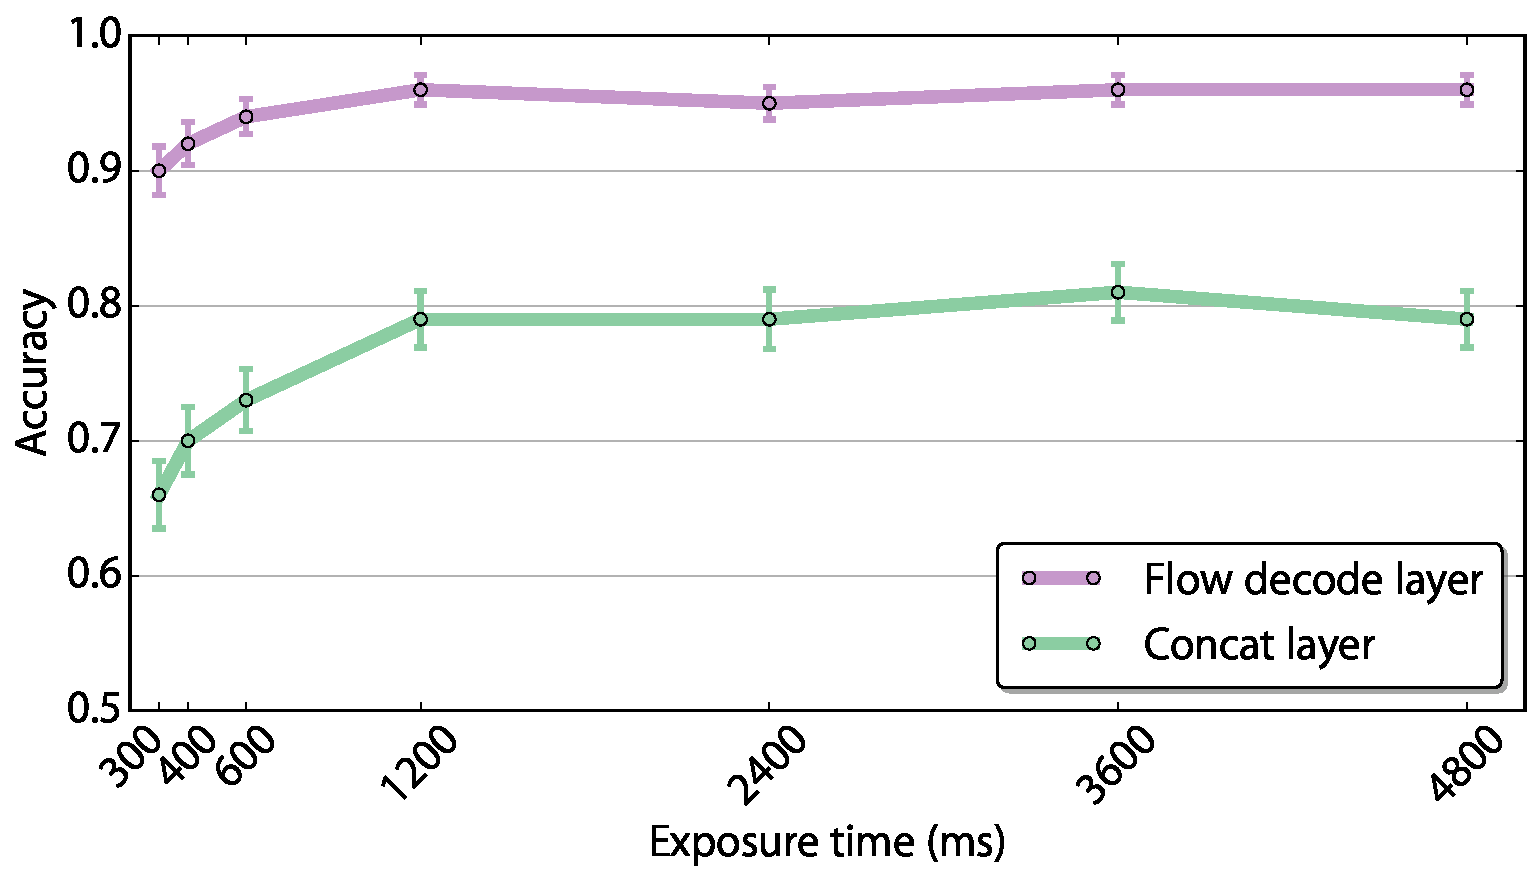
\epsfig{file=alltextures_approvedworkers.pdf, width = 0.9\textwidth}
	\caption[Time-limited pairwise comparisons across all textures]{Time-limited pairwise comparisons across all textures with $95\%$ statistical confidence intervals.}
	\label{fig:pairwise_alltextures}
\end{figure}



A full breakdown of the user study results by dynamic texture and 
grouping can be found in the appendix. \todomatthew{include tables in appendix}
Here some of the overall trends are discussed.

\subsubsection{Appearance-based analysis}

Based on appearance it is clear that textures with
large-scale spatial consistencies (regular, near-regular, 
and irregular textures) tend to perform poorly.
Examples being \path{flag} and \path{fountain_2} with
user accuracies of $98.9\% \pm 1.6\%$ and $90.8\% \pm 4.3\%$ 
averaged across all exposures, respectively.
This is not unexpected and is a fundamental limitation of the 
local nature of the Gram matrix representation used in the 
appearance stream which was observed in static texture synthesis 
\cite{gatys2015}.
In contrast, stochastic and near-stochastic dynamic textures 
performed significantly better as their smaller-scale local 
variations are well captured by the appearance stream, for 
instance \path{water_1} and \path{lava} which had 
average accuracies of $53.8\% \pm 7.4\%$ and
$55.6\% \pm 7.4\%$, respectively, making them both 
statistically indistinguishable from real.

\begin{figure}[t]
	\centering
	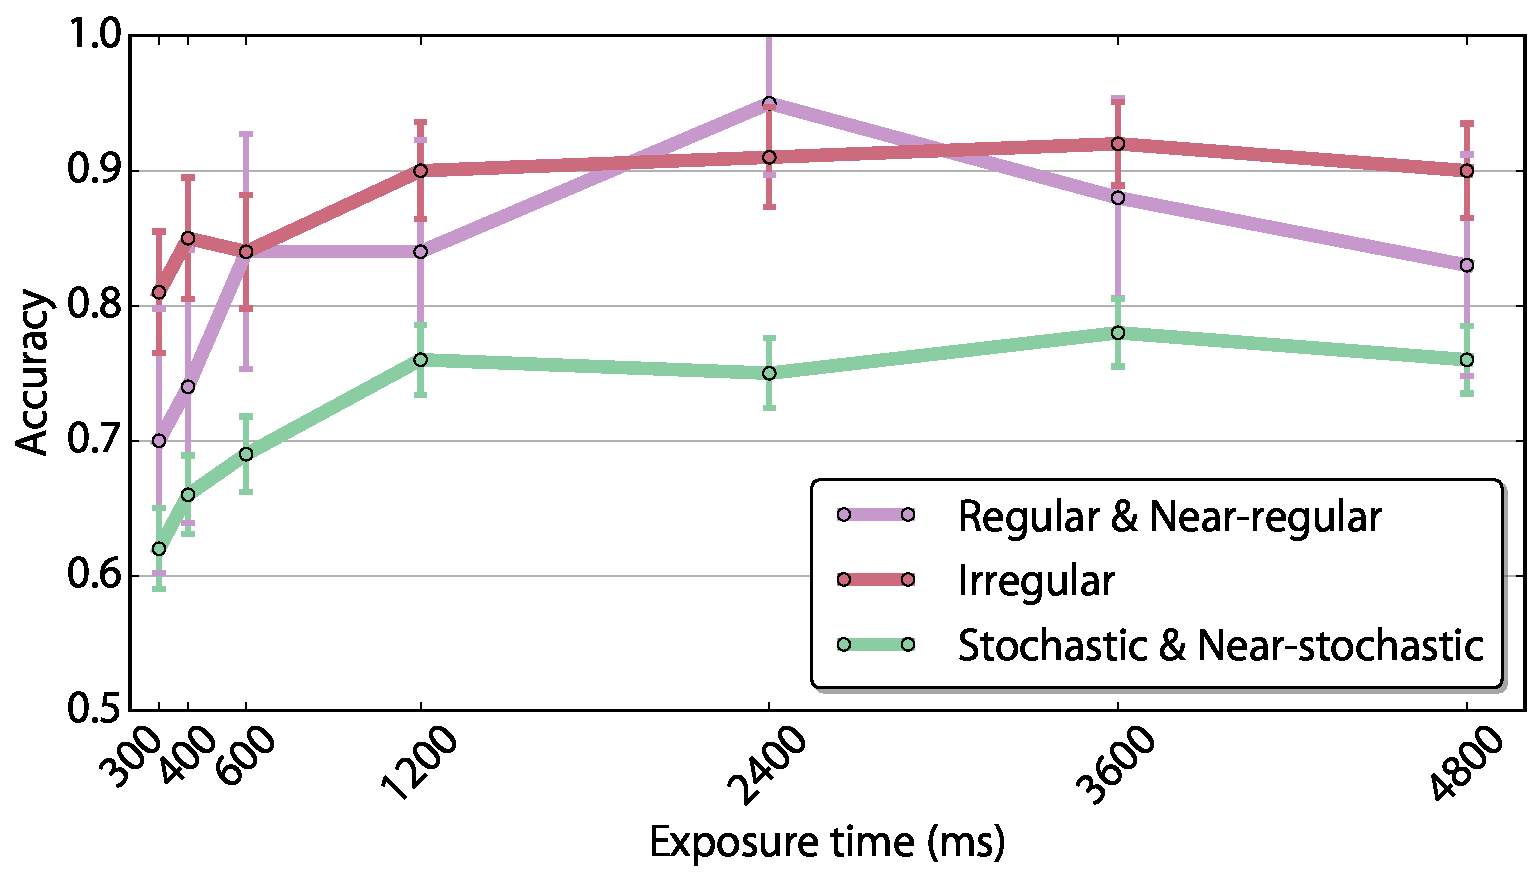
\epsfig{file=concat_appearance.pdf, width = 0.9\textwidth}\\
    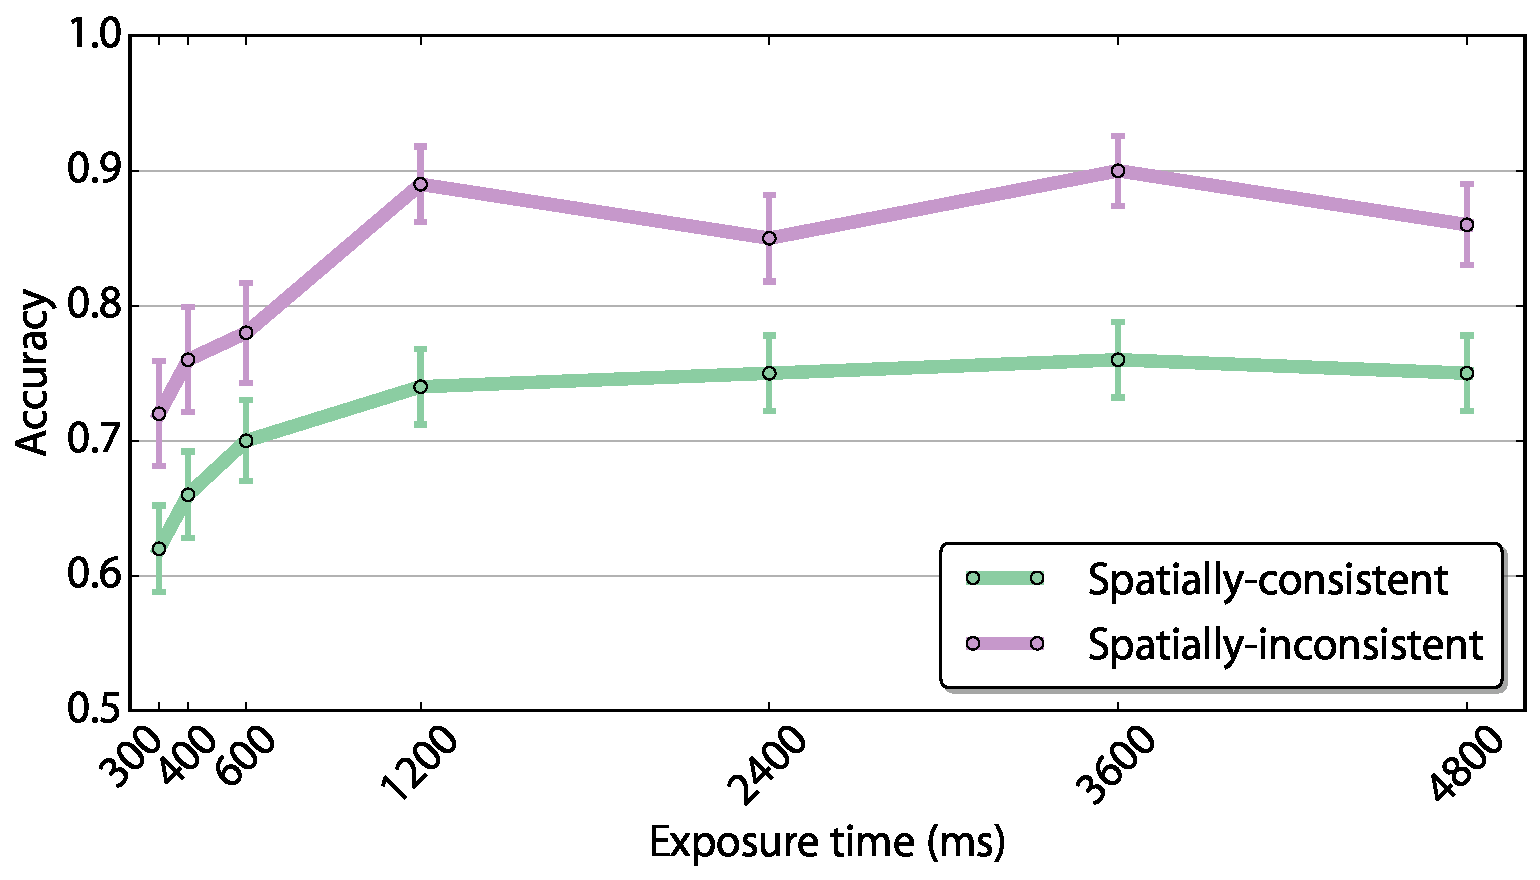
\epsfig{file=concat_dynamics.pdf, width = 0.9\textwidth}
	\caption[Time-limited pairwise comparisons across all textures, grouped by appearance and dynamics.]{Time-limited pairwise comparisons across all textures, grouped by appearance (top) and dynamics (bottom).  Shown with $95\%$ statistical confidence intervals.
	}
	\label{fig:pairwise_grouped}
	\vspace{-0.2cm}
\end{figure}

\subsubsection{Dynamics-based analysis}

In terms of dynamics, the user study showed that textures with
spatially-consistent dynamics (\eg, \path{tv_static}, 
\path{water_*}, and  \path{calm_water_*}) perform 
significantly better than those with spatially-inconsistent 
dynamics (\eg, \path{candle_flame}, \path{fountain_2}, 
and \path{snake_*}), where the dynamics drastically differ 
across spatial locations.
For example, \path{tv_static} and \path{calm_water_6}
have average accuracies of $48.6\% \pm 7.4\%$ and
$63.2\% \pm 7.2\%$, respectively, while
\path{candle_flame} and \path{snake_5} have average 
accuracies of $92.4\% \pm 4\%$ and $92.1\% \pm 4\%$, 
respectively.
Overall, the two-stream model is capable of reproducing a full spectrum
of spatially-consistent dynamics.
However, as the appearance shifts from containing small-scale 
spatial consistencies to containing large-scale spatial consistencies,
performance degrades.
This was evident in the user study where the best-performing 
textures typically consisted of a stochastic or
near-stochastic appearance with spatially-consistent 
dynamics.
In contrast the worst-performing textures consisted of
regular, near-regular, or irregular appearance with
spatially-inconsistent dynamics.

\section{Qualitative comparisons}

In this section, a qualitative comparison with the competing methods of Funke 
\etal \cite{funke2017} and Xie \etal \cite{xie2017synthesizing} is performed. \todomatthew{explain their methods in related work}
Generally, results from the proposed two-stream model are found to be qualitatively comparable or better than these methods.

To note, Funke \etal \cite{funke2017} provided results on
only five textures and of those only four
are dynamic textures in the sense that their appearance
and dynamics are spatiotemporally coherent.
Their results on these sequences (\path{cranberries}, \path{flames}, 
\path{leaves}, and \path{water_5}) are included in the folder
\path{funke} under \path{dynamic_texture_synthesis/comparisons} in the supplementary material.
The results from the two-stream model are included as well.

Results are also compared on nine dynamic textures chosen to cover the full
range of the dynamics and appearance groupings introduced in the user study.
Publicly available code from Funke \etal and Xie \etal is used to produce their
results and the same parameters used in their experiments are used here. For
Funke \etal's model \cite{funke2017}, the parameters used are $\Delta{t}=4$ and
$T=12$ \todomatthew{explain these params} (recall that target dynamic textures
consist of 12 frames). For the spatiotemporal and temporal models from Xie
\etal \cite{xie2017synthesizing}, the parameters used are $T=1200$ and
$\tilde{M}=3$. \todomatthew{explain these params}
A comparison between the results from the proposed two-stream model, Funke
\etal's \cite{funke2017} model, and Xie \etal's \cite{xie2017synthesizing} model
on the nine dynamic textures are included in the folder \path{xie_and_funke}
under \path{dynamic_texture_synthesis/comparisons}. \todomatthew{also include figure}
\todomatthew{maybe leave folder description for appendix}
Note for Xie \etal \cite{xie2017synthesizing}, comparisons are made with their
spatiotemporal model (labeled ``Xie et al.\ (ST)'') designed for dynamic
textures with both spatial and temporal homogeneity, and their temporal model
(labeled ``Xie et al.\ (FC)'') designed for dynamic textures with only temporal
homogeneity.

Overall, the results from the proposed two-stream model appear
qualitatively better, showing more temporal coherence and similarity
in dynamics and fewer artifacts, \eg, blur and flicker.
This may be a natural consequence of the limited representation of dynamics
in both Funke \etal's and Xie \etal's models. Although the spatiotemporal model
of Xie \etal \cite{xie2017synthesizing} is able to synthesize dynamic textures
that lack spatial homogeneity (\eg, \path{bamboo} and \path{escalator}),
note that their method can not synthesize novel dynamic textures, \ie, it
appears to faithfully reproduce the target texture, reducing the applicability
of their approach.

As a consequence of jointly modelling appearance and dynamics, the methods of
\cite{funke2017,xie2017synthesizing} are not capable of the novel form of style
transfer that was demonstrated above. This was enabled by the factored
representation of dynamics and appearance. Furthermore, the spatiotemporal
extent of the output sequence generated by Xie \etal's
\cite{xie2017synthesizing} method is limited to being equal to the input.
The proposed approach does not share this limitation.